%% This is file `elsarticle-template-1-num.tex',
%%
%% Copyright 2009 Elsevier Ltd
%%
%% This file is part of the 'Elsarticle Bundle'.
%% ---------------------------------------------
%%
%% It may be distributed under the conditions of the LaTeX Project Public
%% License, either version 1.2 of this license or (at your option) any
%% later version.  The latest version of this license is in
%%    http://www.latex-project.org/lppl.txt
%% and version 1.2 or later is part of all distributions of LaTeX
%% version 1999/12/01 or later.
%%
%% The list of all files belonging to the 'Elsarticle Bundle' is
%% given in the file `manifest.txt'.
%%
%% Template article for Elsevier's document class `elsarticle'
%% with numbered style bibliographic references
%%
%% $Id: elsarticle-template-1-num.tex 149 2009-10-08 05:01:15Z rishi $
%% $URL: http://lenova.river-valley.com/svn/elsbst/trunk/elsarticle-template-1-num.tex $
%%
\documentclass[preprint,12pt]{elsarticle}

%% Use the option review to obtain double line spacing
%% \documentclass[preprint,review,12pt]{elsarticle}

%% Use the options 1p,twocolumn; 3p; 3p,twocolumn; 5p; or 5p,twocolumn
%% for a journal layout:
%% \documentclass[final,1p,times]{elsarticle}
%% \documentclass[final,1p,times,twocolumn]{elsarticle}
%% \documentclass[final,3p,times]{elsarticle}
%% \documentclass[final,3p,times,twocolumn]{elsarticle}
%% \documentclass[final,5p,times]{elsarticle}
%% \documentclass[final,5p,times,twocolumn]{elsarticle}

%% if you use PostScript figures in your article
%% use the graphics package for simple commands
%% \usepackage{graphics}
%% or use the graphicx package for more complicated commands
%% \usepackage{graphicx}
%% or use the epsfig package if you prefer to use the old commands
%% \usepackage{epsfig}

%% The amssymb package provides various useful mathematical symbols
\usepackage{amssymb}
%% The amsthm package provides extended theorem environments
%% \usepackage{amsthm}

\usepackage{amsmath}
\usepackage{algorithm}
\usepackage[noend]{algpseudocode}
\usepackage{xcolor}
\newcommand\myworries[1]{\textcolor{red}{#1}}
%\usepackage{hyperref}


%% The lineno packages adds line numbers. Start line numbering with
%% \begin{linenumbers}, end it with \end{linenumbers}. Or switch it on
%% for the whole article with \linenumbers after \end{frontmatter}.
\usepackage{lineno}

%% natbib.sty is loaded by default. However, natbib options can be
%% provided with \biboptions{...} command. Following options are
%% valid:

%%   round  -  round parentheses are used (default)
%%   square -  square brackets are used   [option]
%%   curly  -  curly braces are used      {option}
%%   angle  -  angle brackets are used    <option>
%%   semicolon  -  multiple citations separated by semi-colon
%%   colon  - same as semicolon, an earlier confusion
%%   comma  -  separated by comma
%%   numbers-  selects numerical citations
%%   super  -  numerical citations as superscripts
%%   sort   -  sorts multiple citations according to order in ref. list
%%   sort&compress   -  like sort, but also compresses numerical citations
%%   compress - compresses without sorting
%%
%% \biboptions{comma,round}

% \biboptions{}


%\journal{Journal Name}

\makeatletter
\def\BState{\State\hskip-\ALG@thistlm}
\makeatother

\begin{document}

\begin{frontmatter}

%% Title, authors and addresses

%% use the tnoteref command within \title for footnotes;
%% use the tnotetext command for the associated footnote;
%% use the fnref command within \author or \address for footnotes;
%% use the fntext command for the associated footnote;
%% use the corref command within \author for corresponding author footnotes;
%% use the cortext command for the associated footnote;
%% use the ead command for the email address,
%% and the form \ead[url] for the home page:
%%
%% \title{Title\tnoteref{label1}}
%% \tnotetext[label1]{}
%% \author{Name\corref{cor1}\fnref{label2}}
%% \ead{email address}
%% \ead[url]{home page}
%% \fntext[label2]{}
%% \cortext[cor1]{}
%% \address{Address\fnref{label3}}
%% \fntext[label3]{}

\title{Piece-wise quadratic potentials for robust and fast data approximation}

%% use optional labels to link authors explicitly to addresses:
%% \author[label1,label2]{<author name>}
%% \address[label1]{<address>}
%% \address[label2]{<address>}

\author{Alexander N. Gorban, Evgeny M. Mirkes, Andrei Zinovyev}

\address{Leicester, Paris}

\begin{abstract}
Data dimension reduction by constructing low-dimensional approximators is one of the most fundamental approaches in data mining.
Most efficient approximators based on quadratic energy functional are not flexible enough in many circumstances and suffer from sensitivity to outliers,
which led to introducing other functional forms of energy potential that are usually computationally expensive to minimize.
We suggest using piece-wise quadratic energy potentials of subquadratic growth (PQSQ potentials) that can imitate a variety
of approximation metrics used in practice, such as the popular $L1$-norm. A family of subquadratic piece-wise potentials are almost as computationally
efficient in numerical optimization as quadratic ones for the most popular data approximators ($k$-means, principal components, principal graphs),
converge to the global or local energy minimum, allows flexible choice of data approximation metrics and can be naturally
robust to outlier data points. We introduce this family of potentials, provide implementations of several popular data approximators
exploiting them and do benchmarking.
\end{abstract}

\begin{keyword}
data approximation \sep subquadraic potential \sep principal components \sep clustering
%% keywords here, in the form: keyword \sep keyword

%% MSC codes here, in the form: \MSC code \sep code
%% or \MSC[2008] code \sep code (2000 is the default)

\end{keyword}

\end{frontmatter}

%%
%% Start line numbering here if you want
%%
%\linenumbers

%% main text
\section{Introduction}
\label{S:1}

Data dimension reduction by constructing low-dimensional approximators of finite set of vectors is one of the most fundamental approach in data analysis. Starting from the classical data approximators such as $k$-means and linear principal components (PCA), multiple generalizations have been suggested in the last decades (principal manifolds, principal graphs, principal trees, etc.)\cite{Gorban2008Principal}.

We solve the problem of approximating a finite set of vectors ${\vec{x}_i}\in R^m,i=1...N$ (data set) by a simpler object $L$ embedded into the data space, such that for each point $\vec{x}_i$ an approximation error $err(\vec{x}_i,L)$ function can be defined. We assume this function in the form

\begin{equation}\label{distance_function}
err(\vec{x}_i,L) = \min_{y\in L} \sum_k u(x_i^k-y^k),
\end{equation}

\noindent where the upper $k=1...m$ stands for the coordinate index, and $u(x)$ is a monotonously growing symmetrical function, which we will be calling the energy potential. By data approximation we mean that the configuration of $L$ in the data space minimizes the energy

$$
\sum_i err(\vec{x}_i,L) \rightarrow \min.
$$

The simplest form of the energy potential is quadratic $u(x)=x^2$, which leads to the most known data approximators: mean point ($L$ is a point), principal points ($L$ is a set of points) \cite{???}, principal components ($L$ is a line or a hyperplane). In more advanced cases, $L$ can posses some regular properties leading to principal curves ($L$ is a smooth line or spline), principal manifolds ($L$ is a smooth low-dimensional surface) and principal graphs (eg., $L$ is a pluri-harmonic graph embedment) \cite{Gorban2009}.

There exist multiple advantages of using quadratic potential $u(x)$, because it leads to the most computationally efficient algorithms usually based on a splitting schema, a variant of Expectation-Minimization approach \cite{Gorban2009}. For example, $k$-means algorithm solves the problem of finding the set of principal points and the standard iterative Singular Value Decomposition finds principal components. However, quadratic potential is known to be sensitive to outliers in the data set.

Iteratively reweighted least squares \cite{Lu2015}. A Pure L1-norm Principal Component Analysis \cite{Brooks2013}.

\section{Piecewise quadratic potential of subquadratic growth (PQSQ)}
\label{S:2}

\subsection{Definition of the PQSQ potential}

Let us split all non-negative numbers $x\in R_{\geq 0}$ into $p+1$ non-intersecting intervals $R_0=[0;r_1), R_1=[r_1;r_2), ... , R_k=[r_k;r_{k+1}), ..., R_p=[r_p;\infty)$,  for a set of thresholds $r_1<r_2<...<r_p$. For convenience, let us denote $r_0=0, r_{p+1} = \infty$. Piecewise quadratic potential is a continuous monotonously growing function $u(x)$ constructed from pieces of centered at zero parabolas $y=b_k+a_kx^2$, defined on intervals $x\in[r_k,r_{k+1})$ in the following way (see Figure~\ref{potential}):

\begin{equation}\label{PQSQ_f}
u(x)=
\begin{cases}
b_k+a_kx^2, \mbox{if } r_k \leq |x|<r_{k+1}, k=0...p,
\end{cases}
\end{equation}

\begin{equation}\label{PQSQ_acoeffs}
a_k = \frac{f(r_k)-f(r_{k+1})}{r_k^2-r_{k+1}^2},
\end{equation}

\begin{equation}\label{PQSQ_bcoeffs}
b_k = \frac{f(r_{k+1})r_k^2-f(r_{k})r_{k+1}^2}{r_k^2-r_{k+1}^2}
\end{equation}

\noindent where $f(x)$ is the majorating function, which is to be approximated (imitated) by $u(x)$. For example, in the simplest case $f(x)$ can be a linear function : $f(x)=x$, in this case, $\sum_k u(x^k)$ will approximate the $L1$-norm.

Note that accordingly to (\ref{PQSQ_acoeffs},\ref{PQSQ_bcoeffs}), $b_0=0, a_p=0, b_p=f(r_p)$. Therefore, the choice of $r_p$ can naturally create a ``trimmed'' version of energy potential $u(x)$ such that some data points (outliers) would not have any contribution to the gradient of $u(x)$, hence, will not affect the optimization procedure.

The condition of subquadratic growth consists in the requirement $a_{k+1}\leq a_{k}$ and $b_{k+1} \geq b_{k}$. To guarantee this, the following simple condition on $f(x)$ should be satisfied:

\begin{equation}
\label{eq:condition_function}
f'>0, \>\>\> f''x \leq f',
\end{equation}

\noindent i.e., $f(x)$ should grow not faster than any parabola $ax^2+cx, c>0$.

\begin{figure}[h]
\centering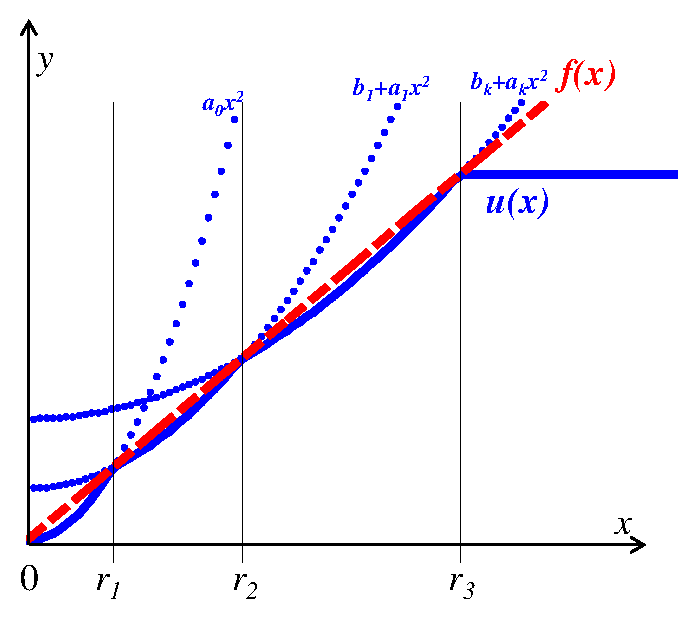
\includegraphics[width=0.6\linewidth]{potential.eps}
\caption{Trimmed piecewise quadratic potential of subquadratic growth $u(x)$ (solid blue line) defined for the majorating function $f(x)$ (red dashed line) and several thresholds $r_k$. Dotted lines shows the parabolas which fragments are used to construct $u(x)$.\label{potential}}
\end{figure}

\subsection{Basic approach for optimization}

The definition of approximation error (\ref{distance_function}) implies that any optimization procedure based on this approximation measure can be done independently for each coordinate. Two auxiliary objects should be pre-computed to apply PQSQ potential in data analysis:

(1) set of $p$ interval thresholds $r_s^k, s=1...p$ for each coordinate $k=1...m$.

(2) Matrix of $a$-coefficients computed by (\ref{PQSQ_acoeffs}) based on interval definitions: $a_s^k$, $s=0...p$, $k=1...m$ separately for each coordinate $k$.

Minimization of PQSQ-based functional consists in two steps:

(1) For each coordinate $k$, assign data point indices into non-overlapping sets $\mathcal{R}_s^k$:

\begin{equation}
\mathcal{R}_s^k= \{i: r_{s}^k \leq |x_i^k-\beta^k_i| < r_{s+1}^k\}, s = 0...p,
\end{equation}

\noindent where $\bf{\beta}$ is a matrix which depends on the nature of the algorithm.

(2) Minimize PQSQ-based functional for each coordinate $k$ independently, where each set of points $\{x_{i\in \mathcal{R}_s^k}\}$ contributes
to the functional quadratically with coefficient $a_s^k$. This is a quadratic optimization task.

(3) Repeat (1)-(2) till convergence which is guaranteed by the definition (\ref{PQSQ_f}) of $u(x)$.


\subsection{Mean value and $k$-means clustering in PQSQ approximation measure}

Mean vector $\bar{X}_L$  for a set of vectors $X=\{x_i^k\}$, $i=1...N, k=1...m$ and an approximation error defined by potential $u(x)$ can be defined as a point minimizing the mean energy potential for all points in  $X$:

\begin{equation}
\sum_i\sum_k f(x_i^k-\bar{X}^k) \rightarrow \min.
\end{equation}

For Euclidean metrics $L_2$ ($u(x)=x^2$) it is the usual arithmetric mean, for $L_1$ metrics ($u(x)=|x|$) this is a vector of median values.

For PQSQ approximation measure (\ref{PQSQ_f}) there is no simple explicit formula for computing the mean value.  In order to find a point $\bar{X}_{PQSQ}$ minimizing mean $PQSQ$ potential, a simple iterative algorithm can be used:

%%\begin{algorithm}
%%\caption{Computing PQSQ mean value}\label{PQSQ_mean}
%%\begin{algorithmic}[1]
%%\Procedure{PQSQ Mean}{}
%%\State $\textit{stringlen} \gets \text{length of }\textit{string}$
%%\State $i \gets \textit{patlen}$
%%\BState \emph{top}:
%%\If {$i > \textit{stringlen}$} \Return false
%%\EndIf
%%\State $j \gets \textit{patlen}$
%%\BState \emph{loop}:
%%\If {$\textit{string}(i) = \textit{path}(j)$}
%%\State $j \gets j-1$.
%%\State $i \gets i-1$.
%%\State \textbf{goto} \emph{loop}.
%%\State \textbf{close};
%%\EndIf
%%\State $i \gets i+\max(\textit{delta}_1(\textit{string}(i)),\textit{delta}_2(j))$.
%%\State \textbf{goto} \emph{top}.
%%\EndProcedure
%%\end{algorithmic}
%%\end{algorithm}

\begin{algorithm}
\caption{Computing PQSQ mean value}\label{PQSQ_Mean_Algorithm}
\begin{algorithmic}[1]
\Procedure{PQSQ Mean Value}{}
\State $\textit{define intervals } r_s^k, s=0...p, k=1...m$
\State $\textit{compute coefficients } a_s^k$
\State $\textit{initialize } \bar{X}_{PQSQ} \textit{ : eg., by arithmetic mean}$
\BState \emph{repeat till convergence of $\bar{X}_{PQSQ}$}:
\State \textbf{for each } \textit{coordinate } $k$
\State \textit{define sets of indices}
$$\mathcal{R}_s^k=\{i: r_{s}^k \leq |x_i^k-\bar{X}_{PQSQ}^k| < r_{s+1}^k\}, s = 0...p $$
\State \textit{compute new approximation for } $\bar{X}_{PQSQ}$:
\State $\bar{X}_{PQSQ}^k \gets \frac{\sum_{s=1...p}a_s^k\sum_{i\in \mathcal{R}_s^k}x_i^k}{\sum_{s=1...p}a_s^k|\mathcal{R}_s^k|}$
\State \textbf{end for}
\State \textbf{goto} \emph{repeat till convergence}
\EndProcedure
\end{algorithmic}
\end{algorithm}

Based on the PQSQ approximation measure and the algorithm for computing the PQSQ mean value (\ref{PQSQ_Mean_Algorithm}), one can construct the PQSQ-based $k$-means clustering procedure in the usual way, splitting estimation of cluster centroids given partitioning of the data points into $k$ disjoint groups, and then re-calculating the partitioning using the PQSQ-based proximity measure.

\subsection{Principal Component Analysis (PCA) in PQSQ metrics}

Accordingly to the classical definition of the first principal component, it is a line best fit to the data set $X$ \cite{Pearson1901On}. Let us define a line in the parametric form $\vec{y}=\vec{V}u+\vec{\delta}$, where $u \in R^1$ is the parameter. Then the first principal component will be defined by vectors $\vec{V}, \vec{\delta}$ satisfying

\begin{equation}
\sum_i\sum_k f(x_i^k-V^ku_i-\delta^k) \rightarrow \min,
\end{equation}

\noindent where

\begin{equation}
u_i = \arg \min_s \sum_k f(x_i^k-V^ks-\delta^k).
\end{equation}

The standard first principal component (PC1) corresponds to $u(x)=x^2$ when the vectors $\vec{V}, \vec{\delta}$ can be found by a simple iterative splitting algorithm for Singular Value Decomposition (SVD). If $X$ does not contain missing values then $\vec{\delta}$ is the vector of arithmetic mean values. By contrast, computing $L1$-based principal components ($u(x)=|x|$) represents a much more challenging optimization problem \cite{Brooks2013}. Several approximative algorithms for computing $L1$-norm PCA have been recently suggested and benchmarked \cite{}. There was no general efficient algorithm suggested for computing PCA in case of arbitrary approximation measure for some monotonous function $u(x)$.

Computing PCA based on PQSQ approximation error is only slightly more complicated than computing the standard $L2$ PCA by SVD. We provide a pseudo-code (\textbf{Algorithm \ref{PQSQ_PC1}}) of a simple iterative algorithm (similar to \textbf{Algorithm \ref{PQSQ_Mean_Algorithm}}) with guaranteed convergence.

\begin{algorithm}
\caption{Computing PQSQ PCA}\label{PQSQ_PC1}
\begin{algorithmic}[1]
\Procedure{PQSQ First Principal Component}{}
\State $\textit{define intervals } r_s^k, s=0...p, k=1...m$
\State $\textit{compute coefficients } a_s^k$
\State $\vec{\delta} \gets \bar{X}_{PQSQ}$
\State $\textit{initialize } \vec{V} \textit{ : eg., by L2-based PC1}$
\State $\textit{initialize } \{u_i\} \textit{ : eg., by } $$u_i = \frac{\sum_k V^k(x_i^k-\delta^k)}{\sum_k (V^k)^2}$$ $
\BState \emph{repeat till convergence of $\vec{V}$}:
\State $\textit{normalize } \vec{V} \textit{ : } \vec{V} \gets \frac{\vec{V}}{||\vec{V}||}$
\State \textbf{for each } \textit{coordinate } $k$
\State \textit{define sets of indices}
$$\mathcal{R}_s^k=\{i: r_{s}^k \leq |x_i^k-V^ku_i-\delta^k| < r_{s+1}^k\}, s = 0...p $$
\State \textbf{end for}
\State \textbf{for each } \textit{data point } $i$ and \textit{coordinate } $k$
%\State \textit{compute new approximation for } $\{u_i\}$:
\State \textit{find all $s_{i,k}$ such that $i\in \mathcal{R}_{s_{i,k}}^k$}
\State \textbf{if}\textit{ all $a^k_{s_{i,k}}=0$ \textbf{then} $t'_i \gets 0$} \textbf{else}
\State
$$u'_i \gets \frac{\sum_{k}a_{s_{i,k}}^kV^k(x_i^k-\delta^k)}{\sum_{k}a_{s_{i,k}}^k(V^k)^2}$$
\State \textbf{end for}
\State \textbf{for each } \textit{coordinate } $k$
%\State \textit{compute new $\vec{V}, \vec{\delta}$}:
%\State \textit{solve $2\times 2$ system of equations for $V^k$, $\delta^k$}:
$$
%\begin{cases}
%V^k \times \sum_s a_s^k \sum_{i\in \mathcal{R}_s^k}u_i + \delta^k \times \sum_s a_s^k |\mathcal{R}_s^k| = \sum_s a_s^k \sum_{i\in \mathcal{R}_s^k}x_i^k \\
%V^k \times \sum_s a_s^k \sum_{i\in \mathcal{R}_s^k}(u_i)^2 + \delta^k \times \sum_s a_s^k \sum_{i\in \mathcal{R}_s^k}u_i = \sum_s a_s^k \sum_{i\in \mathcal{R}_s^k}x_i^ku_i
V^k \gets \frac{\sum_s a_s^k \sum_{i\in \mathcal{R}_s^k}(x_i^k-\delta^k)u_i}{\sum_s a_s^k \sum_{i\in \mathcal{R}_s^k}(u_i)^2}
%\end{cases}
$$
\State \textbf{end for}
\State \textbf{for each } $i$ :
\State $u_i \gets u'_i$
\State \textbf{end for}
\State \textbf{goto} \emph{repeat till convergence}
\EndProcedure
\end{algorithmic}
\end{algorithm}

Computation of second and further principal components follows the standard deflation approach: projections of data points onto the previously computed component are subtracted from the data set, and the algorithm is applied to the residues. However, as it is the case in any non-quadratic metrics, the resulting components can not be orthogonal anymore.
Moreover, unlike $L2$-based principal components, the algorithm \ref{PQSQ_PC1} does not always converge to a unique global minimum; the computed components can depend on the initial estimate of $\vec{V}$. The situation is somewhat similar to the standard $k$-means algorithm. Therefore, in order to achieve the least possible approximation error to the linear subspace, $\vec{V}$ can be initialized randomly or by data vectors $\vec{x}_i$ many times and the deepest in PQSQ approximation error (\ref{distance_function}) minimum should be selected.


\subsection{PQSQ-based Principal Graphs and Manifolds}


\subsection{Convergence properties}


\section{Numerical examples}

\subsection{Practical choices of parameters}

The main parameters of PQSQ are (a) majorating function $f(x)$ and (b) decomposition of each coordinate range into $p+1$ non-overlapping intervals.
Depending on these parameters, various approximation error properties can be exploited, including robustness to outlier data points.

When defining the intervals $r_j, j=1\dots p$, it is desirable to achieve a small difference between $u(\Delta x)-u(\Delta x)$ for expected argument values $\Delta x$ (differences between an estimator and the data points), and choose the suitable value of the potential trimming threshold $r_p$ in order to achieve the desired robustness properties. If no trimming is needed, then $r_p$ should be made larger than the maximum expected difference between coordinate values.

In our numerical experiments we used the following definition of intervals. For any data coordinate $k$, we define a characteristic difference $D^k$, for example

\begin{equation}\label{characteristic_distance_amplitude}
D^k = \alpha_{scale}(max_i(x_i^k)-min_i(x_i^k)),
\end{equation}

\noindent where $\alpha_{scale}$ is a scaling parameter, which can be put at 1 (in this case, the approximating potential will not be trimmed). In case of existence of outliers, for defining $D^k$, instead of amplitude one can use other measures such as the median absolute deviation (MAD):

\begin{equation}\label{characteristic_distance_mad}
D^k = \alpha_{scale}median_i(x_i^k-median(\{x_i^k\}));
\end{equation}

\noindent in this case, the scaling parameter should be made larger, i.e. $\alpha_{scale}=10$, if no trimming is needed.

After defining $D^k$ we use the following definition of intervals:

\begin{equation}\label{intervals_definition}
r_j^k = D^k\frac{j^2}{p^2}, j=0\dots p.
\end{equation}

More sophisticated approaches are also possible to apply such as, given the number of intervals $p$ and the majorating function $f(x)$, choose $r_j, j=1\dots p$ in order to minimize the integral difference

$$
\int_0^{r_p}(f(x)-u(x))dx \rightarrow \min.
$$

In further examples, we use (\ref{characteristic_distance_amplitude}) and (\ref{intervals_definition}) to define intervals in (\ref{PQSQ_f}).

\subsection{Implementation}

At https://github.com/auranic/PQSQ-DataApproximators we provide implementation of PQSQ approximators (in particular, PCA) in Matlab. We also provide Java implementation of PQSQ-based approximators (PCA, principal graphs) as a part of \emph{vdaoengine} library at https://github.com/auranic/VDAOEngine. The code is accompanied by examples of application.




\subsection{Computation performance}

Comparison PQSQ-based PCA with standard quadratic metrics algorithm for computing SVD.

\subsection{Robust principal components, approximating $L1$-based PCA}

Comparison of computation time and precision PQSQ-based PCA for $u(x)=|x|$ with $L1$-based PCA (pcaL1 R implementation by Brooks et al.). See
http://www.optimization-online.org/DB\_FILE/2012/04/3436.pdf for possible benchmarking.




\section{Conclusion}

In this paper we propose a method of constructing the standard data approximators (mean value, $k$-means clustering, principal components, principal graphs)
for arbitrary non-quadratic approximation error with subquadratic growth by using a piecewise-quadratic energy functional (PQSQ potential). These approximators can be computed
by applying quasi-quadratic optimization procedures, which are simple adaptations of the previously described standard and computationally efficient algorithms.

The suggested methodology have several advantages:

(a) \textit{Scalability}: the algorithms are computationally efficient and can be applied to large data sets containing millions of numerical values.

(b) \textit{Flexibility}: the algorithms can be adapted to any type of data metrics with subquadratic growth, even if the metrics can not be expressed in explicit form. Idea of adaptive metrics \cite{Yang2006, Wu2009}.

(c) \textit{Built-in robustness}: choice of intervals in PQSQ can be done in the way to achieve a trimmed version of the standard data approximators, when points distant from the approximator do not affect to the energy minimization during the current optimization step.

(d) \textit{Guaranteed convergence}: the suggested algorithms converge to local or global minimum just as the corresponding predecessor algorithms based on quadratic optimization and expectation/minimization-based splitting approach.

One of the application of the suggested methodology is approximating the popular in data mining $L1$ metrics. \myworries{ Does it provide (more) sparsity also compared to L2?} We show by numerical simulations, that PQSQ-based approximators...

PSQS potential can be evidently applied in the task of regression, replacing the classical Least Squares or L1-based Least Absolute Deviation methods.

\bibliographystyle{model1-num-names}
\bibliography{SubquadraticPotential}

%% Authors are advised to submit their bibtex database files. They are
%% requested to list a bibtex style file in the manuscript if they do
%% not want to use model1-num-names.bst.

%% References without bibTeX database:

% \begin{thebibliography}{00}

%% \bibitem must have the following form:
%%   \bibitem{key}...
%%

% \bibitem{}

% \end{thebibliography}


\end{document}

%%
%% End of file `elsarticle-template-1-num.tex'.
